\documentclass[12pt]{report}
\usepackage[utf8]{inputenc}
\usepackage[russian]{babel}
%\usepackage[14pt]{extsizes}
\usepackage{listings}
\usepackage{amsmath}
\usepackage[justification=centering]{caption}

\lstdefinelanguage{Kotlin}{
  comment=[l]{//},
  commentstyle={\color{gray}\ttfamily},
  emph={delegate, filter, first, firstOrNull, forEach, lazy, map, mapNotNull, println, return@},
  emphstyle={\color{OrangeRed}},
  identifierstyle=\color{black},
  keywords={abstract, actual, as, as?, break, by, class, companion, continue, data, do, dynamic, else, enum, expect, false, final, for, fun, get, if, import, in, interface, internal, is, null, object, override, package, private, public, return, set, super, suspend, this, throw, true, try, typealias, val, var, vararg, when, where, while},
  keywordstyle={\color{blue}\bfseries},
  morecomment=[s]{/*}{*/},
  morestring=[b]",
  morestring=[s]{"""*}{*"""},
  ndkeywords={@Deprecated, @JvmField, @JvmName, @JvmOverloads, @JvmStatic, @JvmSynthetic, Array, Byte, Double, Float, Int, Integer, Iterable, Long, Runnable, Short, String},
  ndkeywordstyle={\color{orange}\bfseries},
  sensitive=true,
  stringstyle={\color{green}\ttfamily},
}

% Для листинга кода:
\lstset{ %
language=Kotlin,                 % выбор языка для подсветки (здесь это С)
basicstyle=\footnotesize\sffamily, % размер и начертание шрифта для подсветки кода
numbers=left,               % где поставить нумерацию строк (слева\справа)
numberstyle=\tiny,           % размер шрифта для номеров строк
stepnumber=1,                   % размер шага между двумя номерами строк
numbersep=5pt,                % как далеко отстоят номера строк от подсвечиваемого кода
showspaces=false,            % показывать или нет пробелы специальными отступами
showstringspaces=false,      % показывать или нет пробелы в строках
showtabs=false,             % показывать или нет табуляцию в строках
frame=single,              % рисовать рамку вокруг кода
tabsize=2,                 % размер табуляции по умолчанию равен 2 пробелам
captionpos=t,              % позиция заголовка вверху [t] или внизу [b] 
breaklines=true,           % автоматически переносить строки (да\нет)
breakatwhitespace=false, % переносить строки только если есть пробел
escapeinside={\#*}{*)}   % если нужно добавить комментарии в коде
}

\usepackage{hyperref}
\hypersetup{
    linktoc=all,     %set to all if you want both sections and subsections linked
    linkcolor=blue,  %choose some color if you want links to stand out
}

% Для измененных титулов глав:
\usepackage{titlesec, blindtext, color} % подключаем нужные пакеты
\definecolor{gray75}{gray}{0.75} % определяем цвет
\newcommand{\hsp}{\hspace{20pt}} % длина линии в 20pt
% titleformat определяет стиль
\titleformat{\chapter}[hang]{\Huge\bfseries}{\thechapter\hsp\textcolor{gray75}{|}\hsp}{0pt}{\Huge\bfseries}

% plot
\usepackage{pgfplots}
\usepackage{filecontents}
\usetikzlibrary{datavisualization}
\usetikzlibrary{datavisualization.formats.functions}
\begin{filecontents}{KA0.dat}
100 2148121
200 17350292
300 68920554
400 211301483
500 367822853
600 678478122
\end{filecontents}

\begin{filecontents}{KV0.dat}
100 2302331
200 22592034
300 73453362
400 205981760
500 351730341
600 658012453
\end{filecontents}

\begin{filecontents}{UKV0.dat}
100 1921005
200 1425033
300 57000923
400 172968826
500 340284336
600 625149992
\end{filecontents}

\begin{filecontents}{KA1.dat}
101 2312114
201 20247410
301 75166547
401 227614782
501 364368768
601 672846913
\end{filecontents}

\begin{filecontents}{KV1.dat}
101 2623891
201 21694235
301 77955778
401 218087162
501 362588416
601 671159157
\end{filecontents}

\begin{filecontents}{UKV1.dat}
101 2032155
201 17554153
301 64421195
401 171881527
501 358108198
601 647843183
\end{filecontents}


\begin{document}
\begin{titlepage}
	\fontsize{12pt}{12pt}\selectfont
	\noindent \begin{minipage}{0.15\textwidth}
		
\includegraphics[width=\linewidth]{inc/img/b_logo.jpg}
	\end{minipage}
	\noindent\begin{minipage}{0.9\textwidth}\centering
		\textbf{Министерство науки и высшего образования Российской Федерации}\\
		\textbf{Федеральное государственное бюджетное образовательное учреждение высшего образования}\\
		\textbf{«Московский государственный технический университет имени Н.Э.~Баумана}\\
		\textbf{(национальный исследовательский университет)»}\\
		\textbf{(МГТУ им. Н.Э.~Баумана)}
	\end{minipage}
	
	\noindent\rule{15cm}{3pt}
	\newline\newline
	\noindent ФАКУЛЬТЕТ \underline{~~~~~~~~~~~~~~~~«Информатика и системы управления»~~~~~~~~~~~~~~~~} \newline\newline
	\noindent КАФЕДРА \underline{«Программное обеспечение ЭВМ и информационные технологии»}\newline\newline\newline\newline\newline\newline\newline
	
	
	\begin{center}
		\Large\textbf{Отчет по лабораторной работе №2 по курсу "Анализ алгоритмов"}\newline
	\end{center}
	
	\noindent\textbf{Тема} \underline{Алгоритм Копперсмита-Винограда}\newline\newline\newline
	\noindent\textbf{Студент} \underline{Якуба Д. В.}\newline\newline
	\noindent\textbf{Группа} \underline{ИУ7-53Б}\newline\newline
	\noindent\textbf{Оценка (баллы)} \underline{~~~~~~~~~~~~~~~~~~~}\newline\newline
	\noindent\textbf{Преподаватели} \underline{Волкова Л.Л., Строганов Ю.В.}\newline
	
	\begin{center}
		\vfill
		Москва~---~\the\year
		~г.
	\end{center}
\end{titlepage}

\tableofcontents

\newpage
\chapter*{Введение}
\addcontentsline{toc}{chapter}{Введение}
\section*{Цели лабораторной работы}
\begin{enumerate}
\item изучение алгоритмов умножения матриц: классического, Копперсмита-Винограда и модифицированного Копперсмита-Винограда;
\item реализация алгоритмов умножения матриц: классического, Копперсмита-Винограда и модифицированного Копперсмита-Винограда;
\item проведение сравнительного анализа трудоёмкости алгоритмов на основе теоретических расчетов и выбранной модели вычислений;
\item сравнительный анализ алгоритмов на основе экспериментальных данных;
\item подготовка отчёта по лабораторной работе.
\end{enumerate}
\section*{Определение}
Алгоритм Копперсмита-Винограда - это алгоритм умножения квадратных матриц, предложенный в 1987 году Д. Копперсмитом и Ш. Виноградом \cite{CoppersmithAndWinograd}. В исходной весрии асимптотическая сложность алгоритма составляла $O(n^{2.3755})$, где $n$ - это размер стороны матрицы. Алгоритм Копперсмита-Винограда с учётом усерии улучшений и доработок в последующие годы, обладает лучшей асимптотикой среди известных алгоритмов умножения матриц.

На практике алгоритм Копперсмита — Винограда не используется, так как он имеет очень большую константу пропорциональности и начинает выигрывать в быстродействии у других известных алгоритмов только для матриц, размер которых превышает память современных компьютеров \cite{RobinsonSara}.
Поэтому пользуются алгоритмом Штрассена по причинам простоты реализации и меньшей константе в оценке трудоемкости \cite{Strassen}.

\chapter{Аналитическая часть}

\section{Классический алгоритм умножения матриц}

Пусть даны две прямоугольные матрицы
\begin{equation}
	A_{lm} = \begin{pmatrix}
		a_{11} & a_{12} & \ldots & a_{1m}\\
		a_{21} & a_{22} & \ldots & a_{2m}\\
		\vdots & \vdots & \ddots & \vdots\\
		a_{l1} & a_{l2} & \ldots & a_{lm}
	\end{pmatrix},
	\quad
	B_{mn} = \begin{pmatrix}
		b_{11} & b_{12} & \ldots & b_{1n}\\
		b_{21} & b_{22} & \ldots & b_{2n}\\
		\vdots & \vdots & \ddots & \vdots\\
		b_{m1} & b_{m2} & \ldots & b_{mn}
	\end{pmatrix},
\end{equation}

тогда матрица $C$
\begin{equation}
	C_{ln} = \begin{pmatrix}
		c_{11} & c_{12} & \ldots & c_{1n}\\
		c_{21} & c_{22} & \ldots & c_{2n}\\
		\vdots & \vdots & \ddots & \vdots\\
		c_{l1} & c_{l2} & \ldots & c_{ln}
	\end{pmatrix},
\end{equation}

где
\begin{equation}
	\label{anal:eq}
	c_{ij} =
	\sum_{r=1}^{m} a_{ir}b_{rj} \quad (i=\overline{1,l}; j=\overline{1,n})
\end{equation}

будет называться произведением матриц $A$ и $B$.

Реализация классического алгоритма умножения двух матриц заключается в реализации вычисления элементов итоговой матрицы по формуле \ref{anal:eq}

\section{Алгоритм Копперсмита-Винограда умножения матриц}
Если посмотреть на результат умножения двух матриц, то видно, что каждый элемент в нем представляет собой скалярное произведение соответствующих строки и столбца исходных матриц.
Можно заметить также, что такое умножение допускает предварительную обработку, позволяющую часть работы выполнить заранее.

Рассмотрим два вектора $V = (v_1, v_2, v_3, v_4)$ и $W = (w_1, w_2, w_3, w_4)$.
Их скалярное произведение равно: $V \cdot W = v_1w_1 + v_2w_2 + v_3w_3 + v_4w_4$, что эквивалентно (\ref{for:new}):
\begin{equation}
    \label{for:new}
    V \cdot W = (v_1 + w_2)(v_2 + w_1) + (v_3 + w_4)(v_4 + w_3) - v_1v_2 - v_3v_4 - w_1w_2 - w_3w_4.
\end{equation}

Несмотря на то, что второе выражение требует вычисления большего количества операций, чем стандартный алгоритм: вместо четырех умножений - шесть, а вместо трех сложений - десять, выражение в правой части последнего равенства допускает предварительную обработку: его части можно вычислить заранее и запомнить для каждой строки первой матрицы и для каждого столбца второй, что позволит для каждого элемента выполнять лишь два умножения и пять сложений, складывая затем только лишь с 2 предварительно посчитанными суммами соседних элементов текущих строк и столбцов.
Из-за того, что операция сложения быстрее операции умножения в ЭВМ, на практике алгоритм должен работать быстрее стандартного \cite{PogorelovVolkova}.

\section*{Вывод}
Были рассмотрены классический алгоритм множения матриц и алгоритм Копперсмита-Винограда умножения матриц. Основное отличие данных алгоритмов заключается в наличии предварительной обработки данных и количестве проводящихся операций умножения.

\newpage

\chapter{Конструкторская часть}
\section{Блок-схема классического алгоритма умножения матриц}
Блок-схема классического алгоритма умножения матриц предоставлена на рисунке \ref{img:classic}
\begin{figure}
\begin{center}
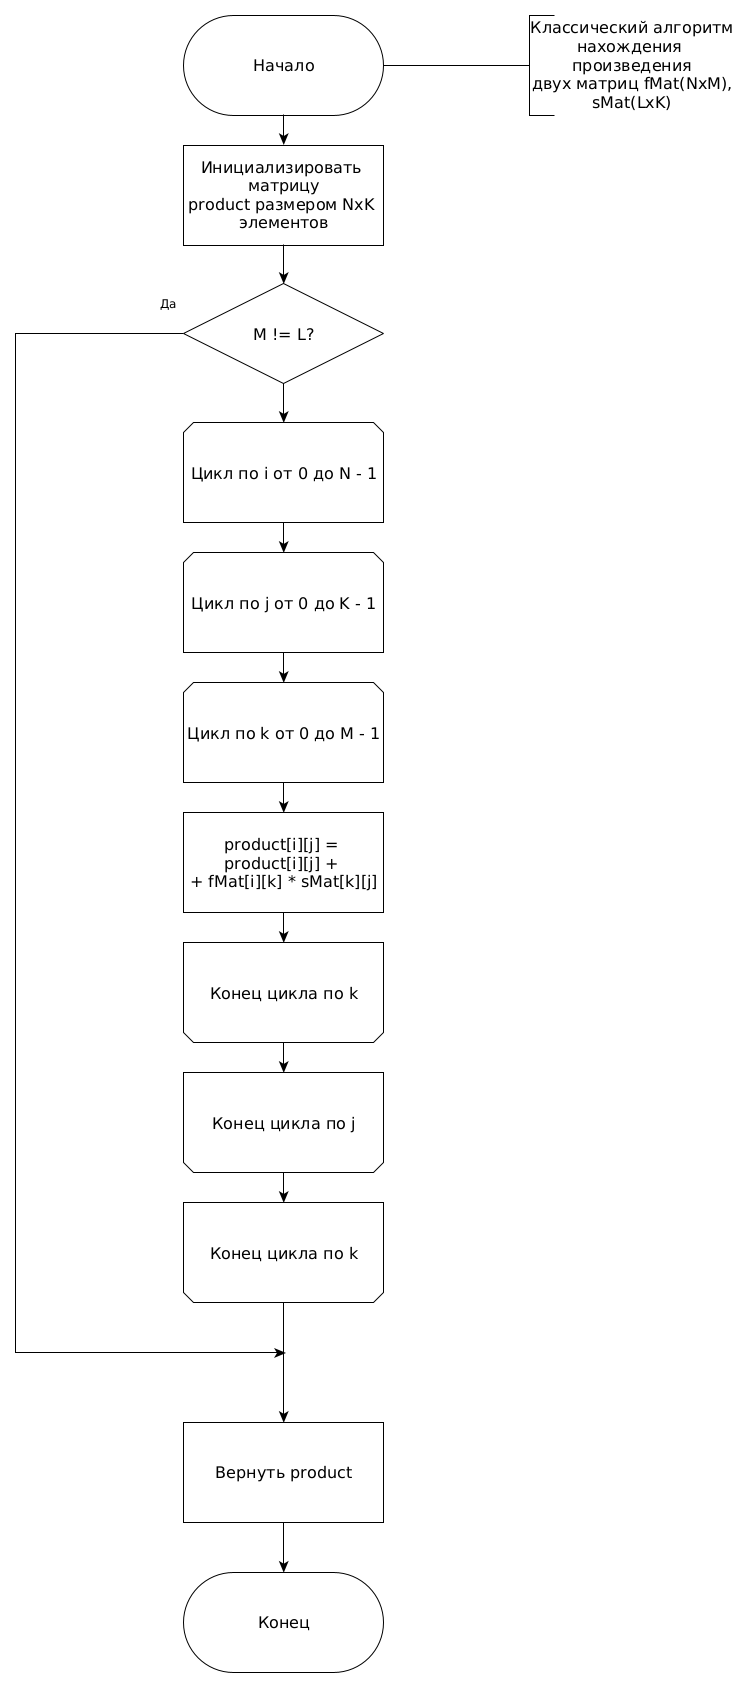
\includegraphics[scale=0.33]{inc/img/classic.png}
\captionsetup{justification=centering}
	\caption{Блок-схема классического алгоритма умножения матрицы.}
	\label{img:classic}	
\end{center}
\end{figure}
\section{Блок-схема алгоритма Копперсмита-Винограда}
Блок-схема алгоритма Копперсмита-Винограда и алгоритмов предвычисления предоставлены на рисунках \ref{img:cols} - \ref{img:Winograd2}.

\begin{figure}
\begin{center}
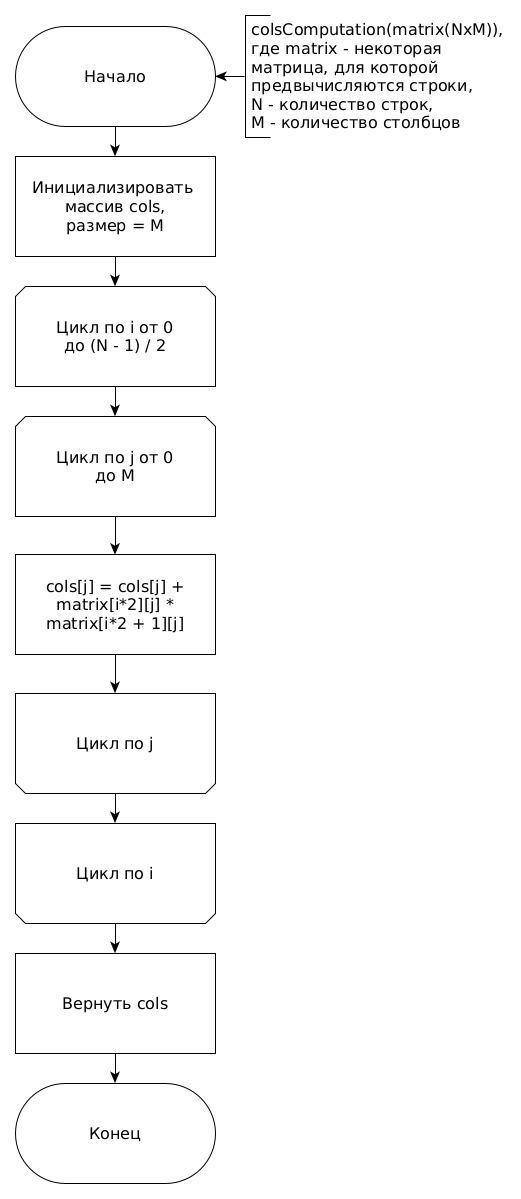
\includegraphics[scale=0.33]{inc/img/colsComp.png}
\captionsetup{justification=centering}
	\caption{Блок-схема алгоритма предвычисления столбцов.}
	\label{img:cols}	
\end{center}
\end{figure}

\begin{figure}
\begin{center}
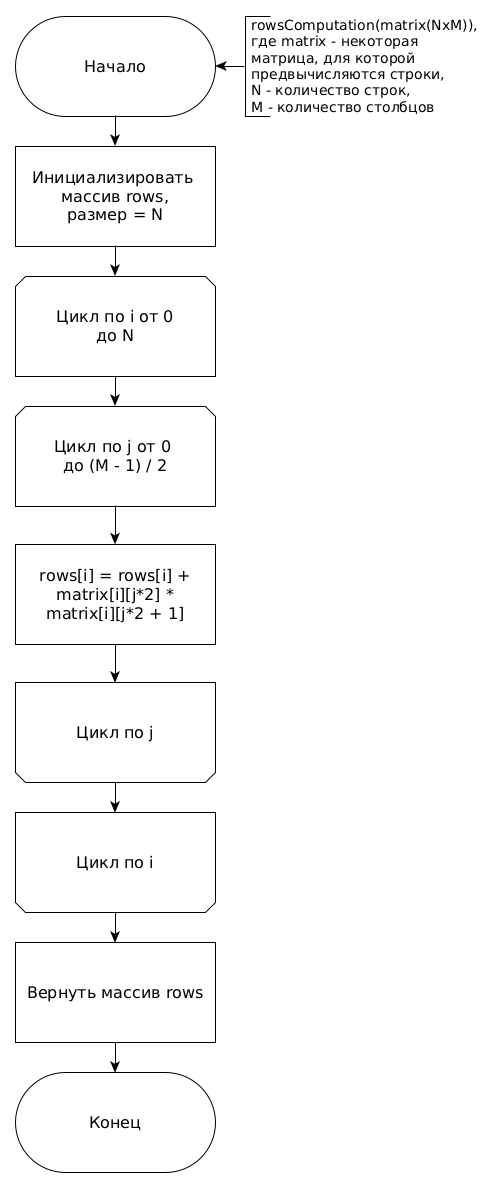
\includegraphics[scale=0.33]{inc/img/rowsComp.png}
\captionsetup{justification=centering}
	\caption{Блок-схема алгоритма предвычисления строк.}
	\label{img:rows}	
\end{center}
\end{figure}

\begin{figure}
\begin{center}
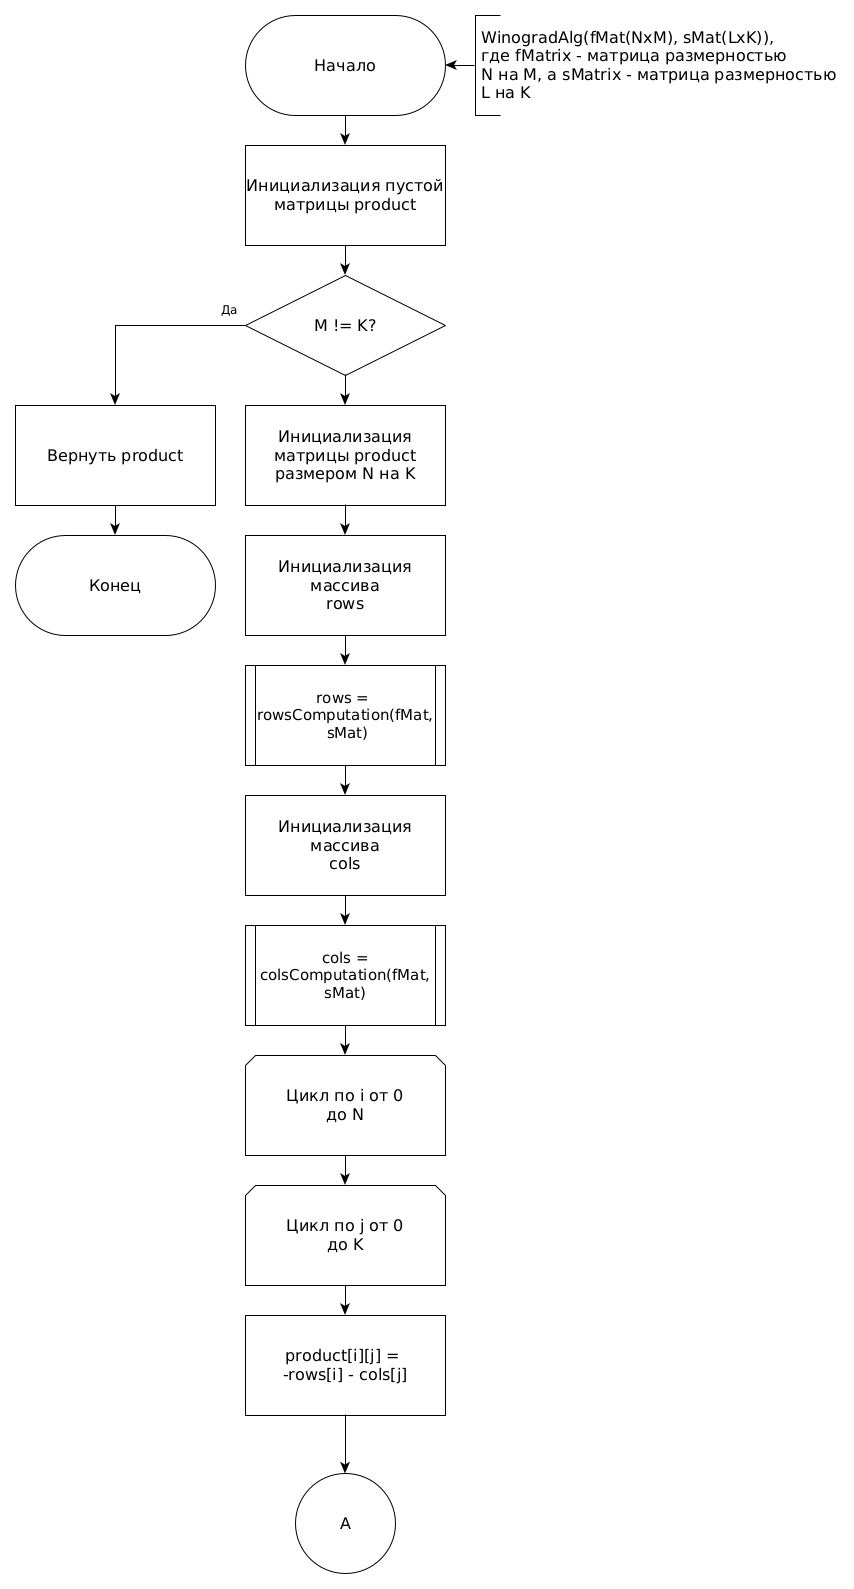
\includegraphics[scale=0.33]{inc/img/Winograd.png}
\captionsetup{justification=centering}
	\caption{Блок-схема алгоритма Копперсмита-Винограда.}
	\label{img:Winograd1}	
\end{center}
\end{figure}

\begin{figure}
\begin{center}
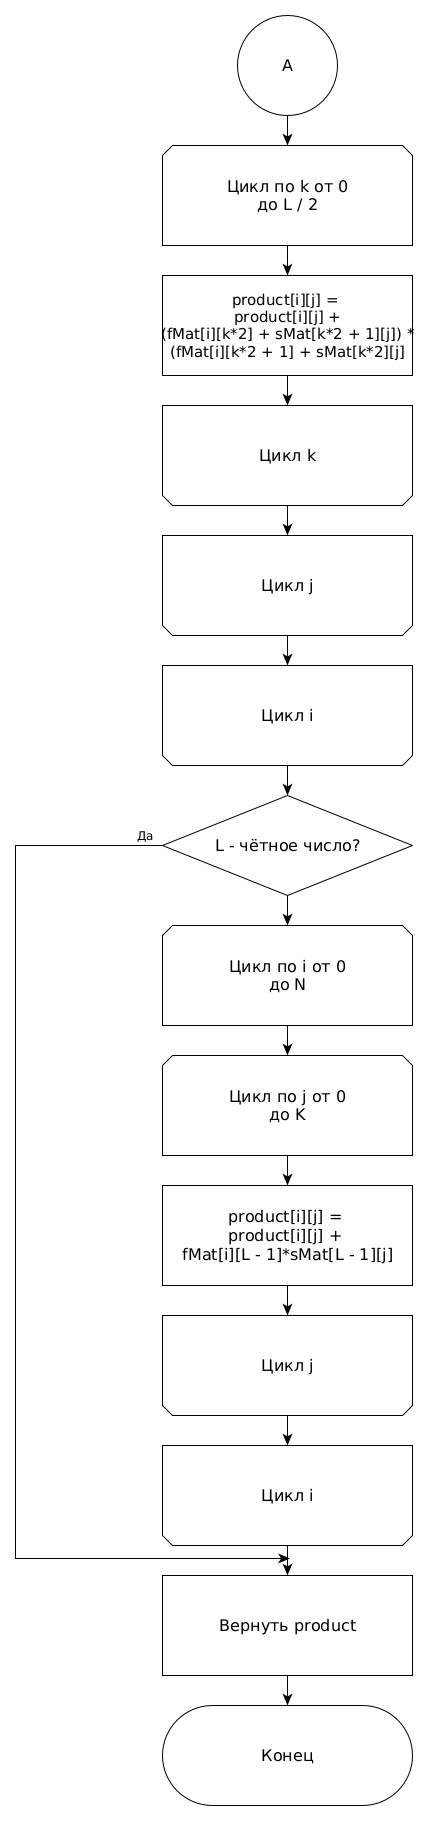
\includegraphics[scale=0.295]{inc/img/WinogradPart2.png}
\captionsetup{justification=centering}
	\caption{Продолжение блок-схемы алгоритма Копперсмита-Винограда.}
	\label{img:Winograd2}	
\end{center}
\end{figure}

\section{Блок-схема улучшенного алгоритма Копперсмита-Винограда}
Блок-схема улучшенного алгоритма Копперсмита-Винограда и алгоритмов предвычисления предоставлены на рисунках \ref{img:colsUpd} - \ref{img:WinogradUpd2}.

\begin{figure}
\begin{center}
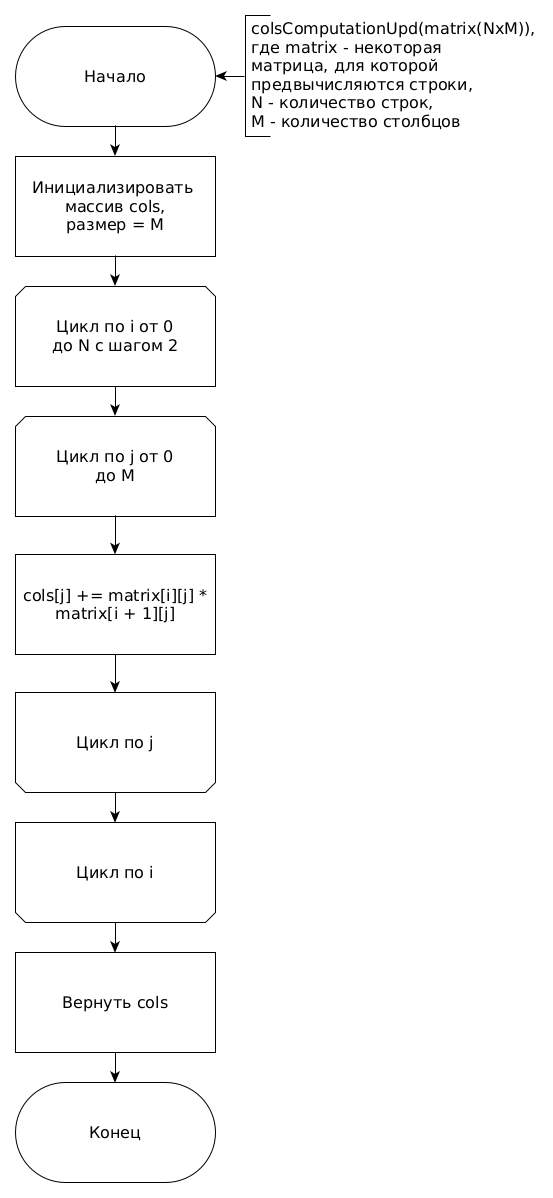
\includegraphics[scale=0.33]{inc/img/colsCompUpd.png}
\captionsetup{justification=centering}
	\caption{Блок-схема алгоритма предвычисления столбцов.}
	\label{img:colsUpd}	
\end{center}
\end{figure}

\begin{figure}
\begin{center}
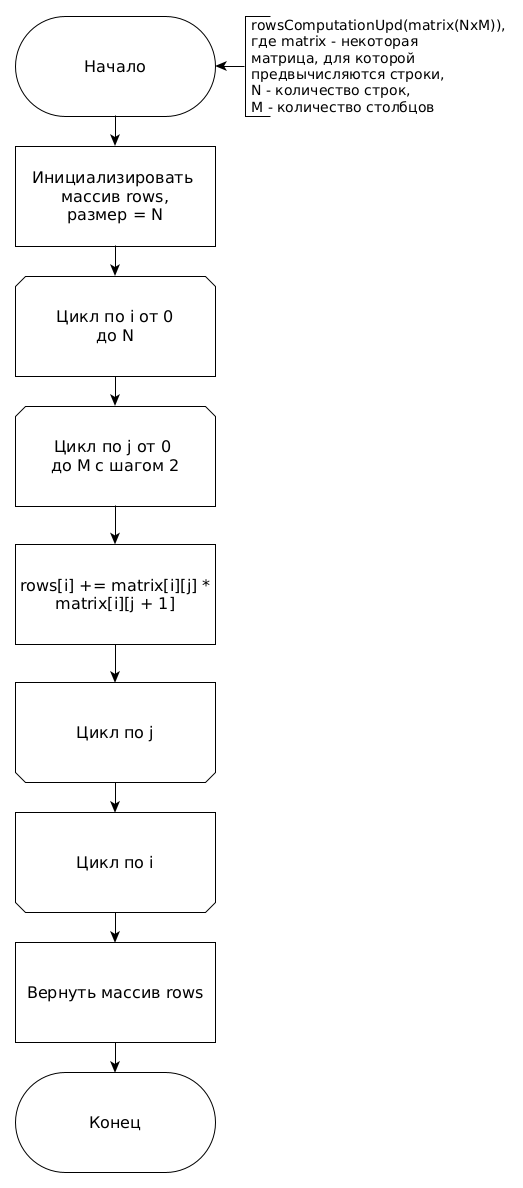
\includegraphics[scale=0.33]{inc/img/rowsCompUpd.png}
\captionsetup{justification=centering}
	\caption{Блок-схема алгоритма предвычисления строк.}
	\label{img:rowsUpd}	
\end{center}
\end{figure}

\begin{figure}
\begin{center}
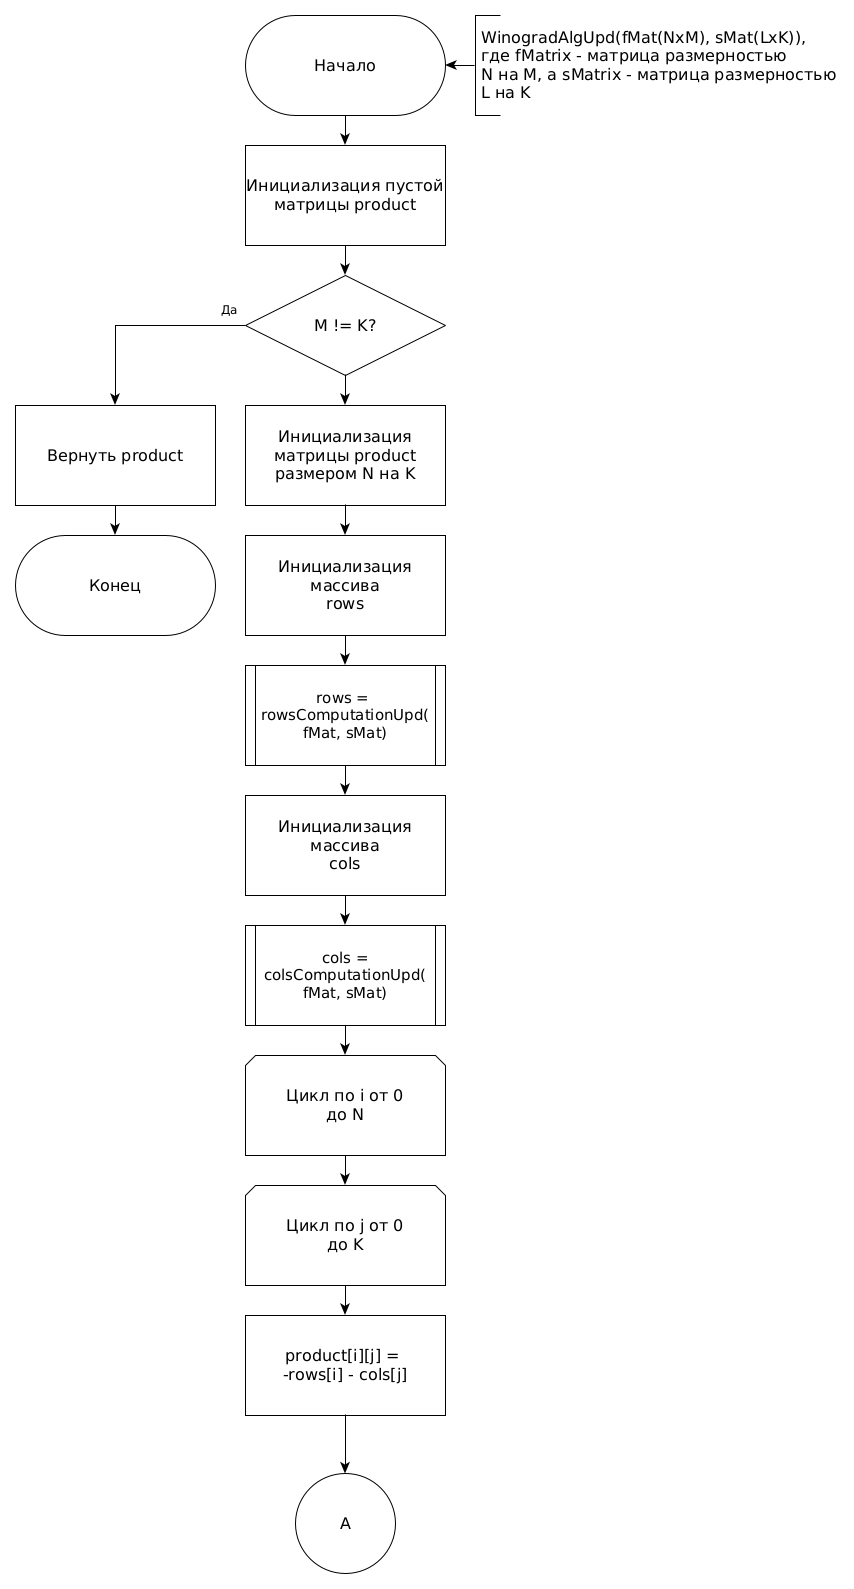
\includegraphics[scale=0.33]{inc/img/WinogradUpd.png}
\captionsetup{justification=centering}
	\caption{Блок-схема улучшенного алгоритма Копперсмита-Винограда.}
	\label{img:WinogradUpd1}	
\end{center}
\end{figure}

\begin{figure}
\begin{center}
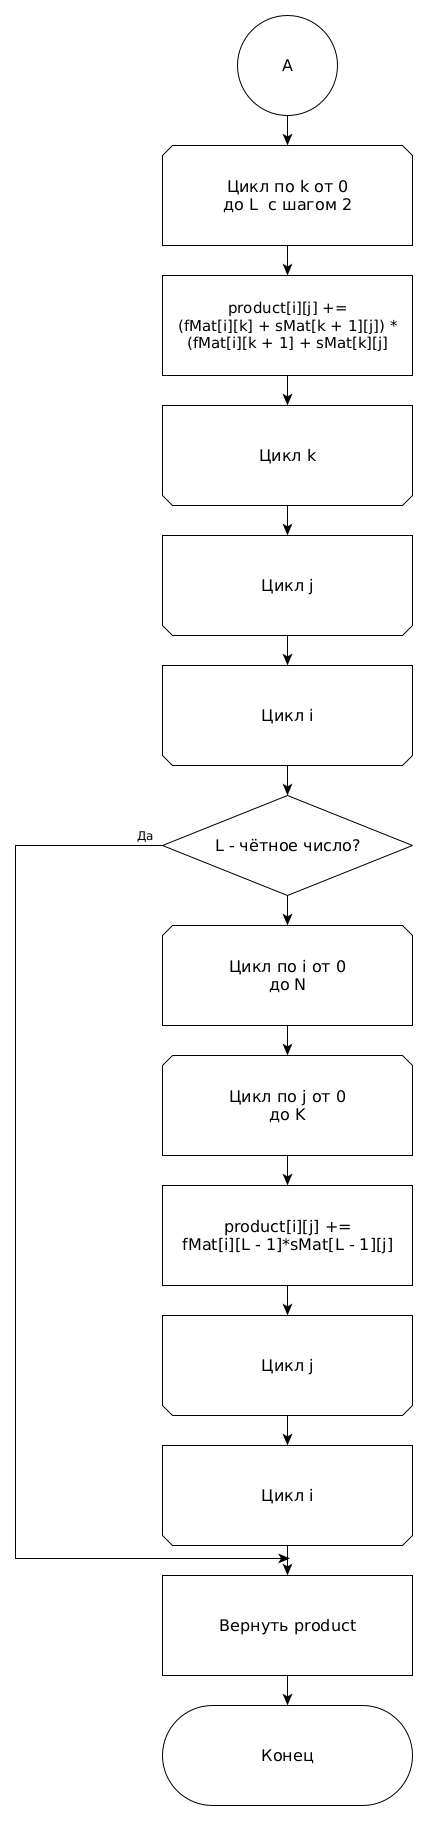
\includegraphics[scale=0.295]{inc/img/WinogradUpdPart2.png}
\captionsetup{justification=centering}
	\caption{Продолжение блок-схемы улучшенного алгоритма Копперсмита-Винограда.}
	\label{img:WinogradUpd2}	
\end{center}
\end{figure}

\newpage
\section{Модель вычислений}

Для последующего вычисления трудоемкости необходимо ввести модель вычислений:
\begin{enumerate}
    \item операции из списка (\ref{operators}) имеют трудоемкость 1;
        \begin{equation}
            \label{operators}
            +, -, /, \%, ==, !=, <, >, <=, >=, [], ++, {-}-, +=, -=
        \end{equation}
    \item трудоемкость оператора выбора \textbf{условие then A else B} рассчитывается, как (\ref{if});
	\begin{equation}
        \label{if}
        f_{if} = f_{\text{условия}} +
        \begin{cases}
        f_A, & \text{если условие выполняется,}\\
        f_B, & \text{иначе.}
        \end{cases}
	\end{equation}
\item трудоемкость цикла рассчитывается, как (\ref{for});
    \begin{equation}
        \label{for:for}
        f_{for} = f_{\text{инициализации}} + f_{\text{сравнения}} + N(f_{\text{тела}} + f_{\text{инкремента}} + f_{\text{сравнения}})
    \end{equation}
	\item трудоемкость вызова функции равна 0.
\end{enumerate}

\section{Трудоёмкость алгоритмов}
\subsection{Классический алгоритм}
Трудоёмкость стандартного алгоритма умножения двух матриц будет включать в себя:
\begin{itemize}
\item Цикл по $i \in [1..N]$, где N - количество строк первой переданной матрицы;
\item Цикл по $j \in [1..K]$, где K - количество столбцов второй переданной матрицы;
\item Цикл по $k \in [1..M]$, где M - количество столбцов первой переданной матрицы.
\end{itemize}

При этом для цикла по $i \in [1..N]$ будем иметь трудоёмкость $f_{i}$ такую, что: $f_{i} = 2 + N \cdot (2 + f_{body})$, где $f_{body}$ - трудоёмкость тела цикла.

Для цикла по $j \in [1..K]$ трудоёмкость $f_{j} = 2 + K \cdot (2 + f_{body})$.

Для цикла по $k \in [1..M]$ трудоёмкость $f_{k} = 2 + 8 \cdot M$.

Как итог, общая трудоёмкость алгоритма может быть представлена выражением \ref{f:fEqu}:
\begin{equation}
\label{f:fEqu}
f = 2 + N \cdot (2 + (2 + K \cdot(2 + 2 + 8 \cdot M)))
\end{equation}

При этом выражение \ref{f:fEqu} преобразуется в \ref{f:sEqu}:
\begin{equation}
\label{f:sEqu}
f = 2 + 4 \cdot N + 4 \cdot K \cdot N + 8 \cdot N \cdot K \cdot M
\end{equation}

\subsection{Алгоритм Копперсмита-Винограда}
Трудоёмкость алгоритма Копперсмита-Винограда умножения двух матриц будет включать в себя:
\begin{itemize}
\item Создание и инициализация массивов $cols$ и $rows$;
\item Заполнение массива $cols$;
\item Заполнение массива $rows$;
\item Цикл заполнения итоговой матрицы для чётных размеров матриц;
\item Цикл для дополнительного заполнения при нечётных размеров матриц;
\end{itemize}

Трудоёмкость создания и инициализации массивов $cols$ и $rows$: $f_{rc} = N + M$, где $M$ - размер массива cols, количество столбцов второй переданной матрицы, а $N$ - размер массива $rows$, количество строк первой переданной матрицы.

Трудоёмкость заполнения массива $cols$: $f_{cols} = 5 + \frac{M - 1}{2}(2 + 11L)$, где $M$ - количество строк второй переданной матрицы, $L$ - количество столбцов второй переданной матрицы.

Трудоёмкость заполнения массива $rows$: $f_{rows} = 2 + N(5 + \frac{M - 1}{2} \cdot 11)$, где $N$ - количество строк первой переданной матрицы, $M$ - количество столбцов первой переданной матрицы.

Трудоёмкость цикла заполнения итоговой матрицы для чётных размеров матриц: $f_{evencyc} = 2 + L(2 + M(9 + 11N))$, где $N$ - количество строк первой матрицы, $M$ - количество столбцов первой матрицы, $L$ - количество столбцов второй матрицы.

Трудоёмкость цикла для дополнительного заполнения при нечётных размерах матриц: $f_{end} = 2 + N(2 + 12L)$. При этом рассматривается два случая, представленных в выражении \ref{end}:

\begin{equation}
	\label{end}
            f_{end} = \begin{cases}
                2, & \text{чётная,}\\
                4 + N(2 + 12L), & \text{иначе.}
            \end{cases}
        \end{equation}
        
Общую формулу для вычисления тудоёмкости можно представить как \ref{endAll}:

\begin{equation}
	\label{endAll}
	f = f_{rc} + f_{cols} + f_{rows} + f_{evencyc} + f_{end}
\end{equation}

Для худшего случая, когда размеры матриц нечётные, из \ref{endAll}:
\begin{equation}
	\label{bad}
	f = 12 +8N + 11N\frac{M - 1}{2} + 2M + 11L\frac{M-1}{2}+ 9NL + 11N^{2}L + 2N + 12NL \approx 11N^{2}L
\end{equation}

Для лучшего случая, когда размеры матриц чётные, из \ref{endAll}:
\begin{equation}
	\label{good}
	f = 10 + 8N + 11N\frac{M - 1}{2} + 2M + 11L\frac{M-1}{2}+ 9NL + 11N^{2}L\approx 11N^{2}L
\end{equation}

\subsection{Улучшенный алгоритм Копперсмита-Винограда}
Трудоёмкость улучшенного алгоритма Копперсмита-Винограда умножения двух матриц будет включать в себя:
\begin{itemize}
\item Создание и инициализация массивов $cols$ и $rows$;
\item Заполнение массива $cols$;
\item Заполнение массива $rows$;
\item Цикл заполнения итоговой матрицы для чётных размеров матриц;
\item Цикл для дополнительного заполнения при нечётных размеров матриц;
\end{itemize}

Трудоёмкость создания и инициализации массивов $cols$ и $rows$: $f_{rc} = N + M$, где $M$ - размер массива cols, количество столбцов второй переданной матрицы, а $N$ - размер массива $rows$, количество строк первой переданной матрицы.

Трудоёмкость заполнения массива $cols$: $f_{cols} = 4 + \frac{M - 1}{2}(2 + 8L)$, где $M$ - количество строк второй переданной матрицы, $L$ - количество столбцов второй переданной матрицы.

Трудоёмкость заполнения массива $rows$: $f_{rows} = 2 + N(4 + \frac{M - 1}{2} \cdot 8)$, где $N$ - количество строк первой переданной матрицы, $M$ - количество столбцов первой переданной матрицы.

Трудоёмкость цикла заполнения итоговой матрицы для чётных размеров матриц: $f_{evencyc} = 2 + L(2 + M(8 + 8N))$, где $N$ - количество строк первой матрицы, $M$ - количество столбцов первой матрицы, $L$ - количество столбцов второй матрицы.

Трудоёмкость цикла для дополнительного заполнения при нечётных размерах матриц: $f_{end} = 2 + N(2 + 10L)$. При этом рассматривается два случая, представленных в выражении \ref{end}:

\begin{equation}
	\label{end2}
            f_{end} = \begin{cases}
                2, & \text{чётная,}\\
                4 + N(2 + 10L), & \text{иначе.}
            \end{cases}
        \end{equation}
        
Общую формулу для вычисления тудоёмкости можно представить как \ref{endAll2}:

\begin{equation}
	\label{endAll2}
	f = f_{rc} + f_{cols} + f_{rows} + f_{evencyc} + f_{end}
\end{equation}

Для худшего случая, когда размеры матриц нечётные, из \ref{endAll2}:
\begin{equation}
	\label{bad2}
	f = M + N + 4 + \frac{M - 1}{2}(2 + 8L) + 2 + N(4 + \frac{M - 1}{2} \cdot 8) + 2 + L(2 + M(8 + 8N)) + 4 + N(2 + 10L) \approx 8MLN
\end{equation}

Для лучшего случая, когда размеры матриц чётные, из \ref{endAll2}:
\begin{equation}
	\label{good2}
	f = M + N + 4 + \frac{M - 1}{2}(2 + 8L) + 2 + N(4 + \frac{M - 1}{2} \cdot 8) + 2 + L(2 + M(8 + 8N)) + 2\approx 8MLN
\end{equation}

\section*{Вывод}
На основе теоретичесих данных, полученных из аналитического раздела, были построены схемы рассматриваемых алгоритмов умноежния матриц, оценены их трудоёмкости в лучшем и худшем случаях.

\chapter{Технологическая часть}
\section{Требования к программному обеспечению}
\begin{itemize}
\item Входные данные - две матрицы размерностью MxN и KxL;
\item Выходые данные - результат умножения двух переданных матриц.
\end{itemize}
\section{Средства реализации программного обеспечения}
При написании программного продукта был использован язык программирования Kotlin \cite{Kotlin}.

Данный выбор обусловлен следующими факторами:
\begin{itemize}
\item Высокая вычислительная производительность;
\item Большое количество справочной литературы, связанной с ЯП Java.
\end{itemize}

Для тестирования производительности реализаций алгоритмов использовалась утилита measureNanoTime.

При написаннии программного продукта использовалась среда разработки IntelliJ IDEA.

Данный выбор обусловлен тем, что язык программирования Kotlin - это разработка компании JetBrains, поставляющей данную среду разработки.

\section{Листинг кода}
В листингах \ref{classic} - \ref{WinogradUpd} предоставлены реализации рассматриваемых алгоритмов.
\begin{lstlisting}[caption=Функция реализации алгоритма классического умножения матриц,
label={classic}]
fun matricesMult(fMatrix: Array<IntArray>, sMatrix: Array<IntArray>) : Array<IntArray>
{
    if (fMatrix[0].size != sMatrix.size)
        return emptyArray()

    val product = Array(fMatrix.size) { IntArray(sMatrix[0].size) }
    for (i in fMatrix.indices)
        for (j in sMatrix[0].indices)
            for (k in fMatrix[0].indices)
                product[i][j] += fMatrix[i][k] * sMatrix[k][j]
    return product
}
\end{lstlisting}

\begin{lstlisting}[caption=Функция реализации алгоритма Копперсмита-Винограда,
label={Winograd}]
fun rowsComputation(matrix: Array<IntArray>) : IntArray
{
    val computedRows = IntArray(matrix.size)

    for (i in matrix.indices)
        for (j in 0 until (matrix[0].size - 1) / 2)
            computedRows[i] = computedRows[i] + matrix[i][j * 2] * matrix[i][j * 2 + 1]

    return computedRows
}

fun colsComputation(matrix: Array<IntArray>) : IntArray
{
    val computedCols = IntArray(matrix[0].size)

    for (i in 0 until (matrix.size - 1) / 2)
        for (j in matrix[0].indices)
            computedCols[j] = computedCols[j] + matrix[i * 2][j] * matrix[i * 2 + 1][j]

    return computedCols
}

fun WinogradMultiplication(fMatrix: Array<IntArray>, sMatrix: Array<IntArray>) : Array<IntArray>
{
    if (fMatrix[0].size != sMatrix.size)
        return emptyArray()

    val computedRows = rowsComputation(fMatrix)
    val computedCols = colsComputation(sMatrix)

    val product = Array(fMatrix.size) { IntArray(sMatrix[0].size) }
    for (i in product.indices)
        for (j in product[0].indices)
        {
            product[i][j] = -computedRows[i] - computedCols[j]

            for (k in 0 until (sMatrix.size / 2))
                product[i][j] = product[i][j] + (fMatrix[i][k * 2] + sMatrix[k * 2 + 1][j]) * (fMatrix[i][k * 2 + 1] + sMatrix[k * 2][j])
        }

    if (sMatrix.size % 2 != 0)
    {
        for (i in product.indices)
            for (j in product[0].indices)
                product[i][j] = product[i][j] + fMatrix[i][sMatrix.size - 1] * sMatrix[sMatrix.size - 1][j]
    }

    return product
}
\end{lstlisting}

\begin{lstlisting}[caption=Функция реализации улучшенного алгоритма Копперсмита-Винограда,
label={WinogradUpd}]
fun rowsComputationModified(matrix: Array<IntArray>) : IntArray
{
    val computedRows = IntArray(matrix.size)
    for (i in matrix.indices)
        for (j in matrix[0].indices step 2)
            computedRows[i] += matrix[i][j] * matrix[i][j + 1]

    return computedRows
}

fun colsComputationModified(matrix: Array<IntArray>) : IntArray
{
    val computedCols = IntArray(matrix[0].size)

    for (i in matrix.indices step 2)
        for (j in matrix[0].indices)
            computedCols[j] += matrix[i][j] * matrix[i + 1][j]

    return computedCols
}

fun WinogradMultiplicationModified(fMatrix: Array<IntArray>, sMatrix: Array<IntArray>) : Array<IntArray>
{
    if (fMatrix[0].size != sMatrix.size)
        return emptyArray()

    val computedRows = rowsComputationModified(fMatrix)
    val computedCols = colsComputationModified(sMatrix)

    val product = Array(fMatrix.size) { IntArray(sMatrix[0].size) }
    for (i in product.indices)
        for (j in product[0].indices)
        {
            product[i][j] = -computedRows[i] - computedCols[j]

            for (k in 0 until (sMatrix.size - 1) step 2)
                product[i][j] += (fMatrix[i][k] + sMatrix[k + 1][j]) * (fMatrix[i][k + 1] + sMatrix[k][j])
        }

    if (sMatrix.size % 2 != 0)
    {
        for (i in product.indices)
            for (j in product[0].indices)
                product[i][j] += fMatrix[i][sMatrix.size - 1] * sMatrix[sMatrix.size - 1][j]
    }

    return product
}
\end{lstlisting}

\section{Тестирование программного продукта}
В таблице~\ref{tabular:test_rec} приведены тесты для функций, реализующих стандартный алгоритм умножения матриц, алгоритм Копперсмита-Винограда и оптимизированный алгоритм Копперсмита-Винограда. Тесты пройдены успешно.

\begin{table}[h!]
	\begin{center}
		\begin{tabular}{c@{\hspace{7mm}}c@{\hspace{7mm}}c@{\hspace{7mm}}c@{\hspace{7mm}}c@{\hspace{7mm}}c@{\hspace{7mm}}}
			\hline
			Матрица 1 & Матрица 2 &Ожидаемый результат \\ \hline
			\vspace{4mm}
			$\begin{pmatrix}
			1 & 2 & 3\\
			1 & 2 & 3\\
			1 & 1 & 1
			\end{pmatrix}$ &
			$\begin{pmatrix}
			1 & 3 & 3\\
			1 & 3 & 3\\
			1 & 2 & 2
			\end{pmatrix}$ &
			$\begin{pmatrix}
			6 & 15 & 15\\
			6 & 15 & 15\\
			3 & 8 & 8
			\end{pmatrix}$ \\
			\vspace{2mm}
			\vspace{2mm}
			$\begin{pmatrix}
            1 & 2 & 4\\
            1 & 2 & 4
			\end{pmatrix}$ &
			$\begin{pmatrix}
			4\\
			5\\
            6
			\end{pmatrix}$ &
			$\begin{pmatrix}
			32\\
			32
			\end{pmatrix}$ \\
			\vspace{2mm}
			\vspace{2mm}
			$\begin{pmatrix}
			5
			\end{pmatrix}$ &
			$\begin{pmatrix}
			666
			\end{pmatrix}$ &
			$\begin{pmatrix}
			3330
			\end{pmatrix}$ \\
			\vspace{2mm}
			\vspace{2mm}
			$\begin{pmatrix}
			-1 & -2 & 3\\
			1 & 2 & 3\\
			-1 & -2 & 3
			\end{pmatrix}$ &
			$\begin{pmatrix}
			1 & 1 & 1\\
			2 & 2 & 2\\
			3 & 3 & 3
			\end{pmatrix}$ &
			$\begin{pmatrix}
			4 & 4 & 4\\
			14 & 14 & 14\\
			4 & 4 & 4
			\end{pmatrix}$\\
			\vspace{2mm}
			\vspace{2mm}
			$\begin{pmatrix}
			666 & 666
			\end{pmatrix}$ &
			$\begin{pmatrix}
			777 & 777
			\end{pmatrix}$ &
			Ошибка\\
		\end{tabular}
	\end{center}
	\caption{\label{tabular:test_rec} Тестирование функций}
\end{table}

\section*{Вывод}
Спроектированные алгоритмы вычисления произведения двух матриц были реализованы и протестированы.

\chapter{Исследовательская часть}

\section{Пример работы программного обеспечения}
Ниже на рисунках \ref{img:exampleRand}- \ref{img:exampleInp} предоставлены примеры работы каждого из алгоритмов на случайных данных, сгенерированных один раз, и введённых пользователем данных:

\begin{figure}
\begin{center}
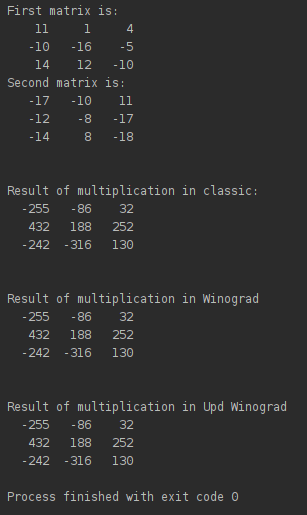
\includegraphics[scale=1]{inc/img/randExample.png}
\captionsetup{justification=centering}
	\caption{Пример работы ПО.}
	\label{img:exampleRand}	
\end{center}
\end{figure}

\begin{figure}
\begin{center}
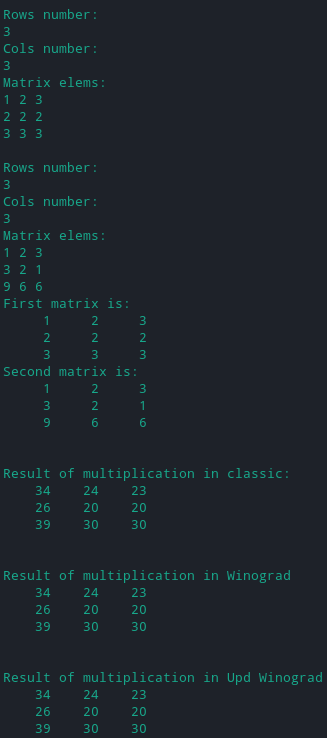
\includegraphics[scale=0.9]{inc/img/inpExample.png}
\captionsetup{justification=centering}
	\caption{Пример работы ПО.}
	\label{img:exampleInp}	
\end{center}
\end{figure}

\newpage

\section{Технические характеристики}
Технические характеристики ЭВМ, на котором выполнялись исследования:
\begin{itemize}
\item ОС: Manjaro Linux 20.1.1 Mikah
\item Оперативная память: 16 Гб
\item Процессор: Intel Core i7-10510U

При проведении замеров времени ноутбук был подключен к сети электропитания.
\end{itemize}

\section{Время выполнения алгоритмов}
Алгоритмы тестировались на данных, сгенерированных случайным образом один раз.

Результаты замеров времени приведены в таблице \ref{time}. На рисунках \ref{timeRes1} и \ref{timeRes2} приведены графики зависимостей времени работы алгоритмов от количества строк и столбцов матриц (в чётном и нечётном вариантах). В таблице КА - Классический Алгоритм, КВ - Алгоритм Копперсмита-Винограда, УКВ - Улучшенный Алгоритм Копперсмита-Винограда.

\newpage
\begin{table}[h]
	\begin{center}
		\caption{\label{time} Замеры времени для квадратных матриц различных размеров}
		\begin{tabular}{|c c c c|} 
 			\hline
			Размер матрицы & КА & КВ & УКВ \\ [0.5ex] 
 			\hline\hline
 			100 & 2148121& 2302331& 1921005\\
 			\hline
 			101 & 2312114& 2623891& 2032155\\
 			\hline
			200 & 17350292& 22592034& 1425033\\
			\hline
			201 & 20247410& 21694235& 17554153\\
			\hline
			300 & 68920554&  73453362& 57000923\\
			\hline
			301 &  75166547&  77955778& 64421195\\
			\hline
			400 &  211301483&  205981760& 172968826\\
			\hline
			401 &  227614782&  218087162& 171881527\\
			\hline
			500 &  367822853&  351730341& 340284336\\
			\hline
			501 &  364368768&  362588416& 358108198\\
			\hline
			600 &  678478122&  	658012453& 625149992\\
			\hline
			601 &  672846913&  671159157& 647843183\\
			\hline
			\end{tabular}
	\end{center}
\end{table}

\begin{figure}[h]
\begin{center}
	\begin{tikzpicture}

\begin{axis}[
  		  	axis lines = left,
  		  	xlabel = $размер$,
  		  	ylabel = {$время$},
			legend pos=north west,
			ymajorgrids=true
		] 
		\addplot[color=orange] table[x index=0, y index=1] {KA0.dat};
		\addplot[color=blue, mark=square] table[x index=0, y index=1] {KV0.dat};
		\addplot[color=green, mark=square] table[x index=0, y index=1] {UKV0.dat};

		\addlegendentry{КА}
		\addlegendentry{КВ}
		\addlegendentry{УКВ}
		\end{axis}
	\end{tikzpicture}
	\captionsetup{justification=centering}
	\caption{Зависимость времени работы от размера матриц (чётные значения размерностей)}
	\label{timeRes1}
	\end{center}
\end{figure}

\begin{figure}[h]
	\begin{center}
	\begin{tikzpicture}

		\begin{axis}[
 		   	axis lines = left,
 		   	xlabel = $размер$,
 		   	ylabel = {$время$},
			legend pos=north west,
			ymajorgrids=true
		]
		\addplot[color=orange] table[x index=0, y index=1] {KA1.dat};
		\addplot[color=blue, mark=square] table[x index=0, y index=1] {KV1.dat};
		\addplot[color=green, mark=square] table[x index=0, y index=1] {UKV1.dat};

		\addlegendentry{КА}
		\addlegendentry{КВ}
		\addlegendentry{УКВ}
		\end{axis}
\end{tikzpicture}
	\captionsetup{justification=centering}
	\caption{Зависимость времени работы от размера матриц (нечётные значения размерностей)}
	\label{timeRes2}
	\end{center}
\end{figure}

\section*{Вывод}
При сравнении результатов замеров времени заметно, что скорость работы классического алгоритма однозначно отстаёт от скорости работы улучшенного Алгоритма Копперсмита-Винограда. Уже на 600 элементах улучшенный алгоритм Копперсмита-Винограда работает быстрее классического на $\approx8\%$. При нечётном количестве строк и столбцов матриц улучшенный алгоритм способен быть медленнее $\approx4\%$, при факте того, что классический алгоритм похожей динамики не имеет. Обычный алгоритм Копперсмита-Винограда начинает выигрывать по скорости классический только по достижению 300 строк и столбцов в матрице, при факте того, что в случае матрицы с нечётной размерностью он всё ещё будет проигрывать. При размерности 600 он будет выгрывать у классической реализации на $\approx3\%$. В случае матриц размера меньше 400 на 400 его использование не будет целесообразным.

\chapter*{Заключение}
\addcontentsline{toc}{chapter}{Заключение}
В ходе выполнения лабораторной работы:
\begin{itemize}
\item были изучены алгоритмы умножения матриц: классический, Копперсмита-Винограда и улучшенный Копперсмита-Винограда;
\item были реализованы алгоритмы умножения матриц: классический, Копперсмита-Винограда и улучшенный Копперсмита-Винограда;
\item был произведён анализ трудоёмкости указанных алгоритмов на основе теоретических расчётов и выбранной модели вычислений;
\item был выполнен сравнительный анализ производительности алгоритмов на основе полученных экспериментальных данных;
\item был подготовлен отчёт по проделанной работе;
\item Были получены практические навыки реализации алгоритмов на ЯП Kotlin.
\end{itemize}

Исследования показали, что использование алгоритма Копперсмита-Винограда способно оправдать себя только в случае матриц, размерность которых не менее 400. При этом выигрыш будет составлять $\approx0.02\%$ только в случае чётной размерности. Реализация улучшенного алгоритма Копперсмита-Винограда показывает быстрее классического алгоритма уже при размерности матрицы 100. Чем больше элементов в матрице - тем заметнее разница во времени работы этих двух алгоритмов.

\addcontentsline{toc}{chapter}{Литература}
\bibliographystyle{utf8gost705u}  % стилевой файл для оформления по ГОСТу
\bibliography{biblio.bib}          % имя библиографической базы (bib-файла)


\end{document} 
